\documentclass[]{article}
\usepackage{lmodern}
\usepackage{amssymb,amsmath}
\usepackage{ifxetex,ifluatex}
\usepackage{fixltx2e} % provides \textsubscript
\ifnum 0\ifxetex 1\fi\ifluatex 1\fi=0 % if pdftex
  \usepackage[T1]{fontenc}
  \usepackage[utf8]{inputenc}
\else % if luatex or xelatex
  \ifxetex
    \usepackage{mathspec}
  \else
    \usepackage{fontspec}
  \fi
  \defaultfontfeatures{Ligatures=TeX,Scale=MatchLowercase}
\fi
% use upquote if available, for straight quotes in verbatim environments
\IfFileExists{upquote.sty}{\usepackage{upquote}}{}
% use microtype if available
\IfFileExists{microtype.sty}{%
\usepackage{microtype}
\UseMicrotypeSet[protrusion]{basicmath} % disable protrusion for tt fonts
}{}
\usepackage[margin=1in]{geometry}
\usepackage{hyperref}
\hypersetup{unicode=true,
            pdftitle={Forecasting Australian GDP},
            pdfborder={0 0 0},
            breaklinks=true}
\urlstyle{same}  % don't use monospace font for urls
\usepackage{color}
\usepackage{fancyvrb}
\newcommand{\VerbBar}{|}
\newcommand{\VERB}{\Verb[commandchars=\\\{\}]}
\DefineVerbatimEnvironment{Highlighting}{Verbatim}{commandchars=\\\{\}}
% Add ',fontsize=\small' for more characters per line
\usepackage{framed}
\definecolor{shadecolor}{RGB}{248,248,248}
\newenvironment{Shaded}{\begin{snugshade}}{\end{snugshade}}
\newcommand{\KeywordTok}[1]{\textcolor[rgb]{0.13,0.29,0.53}{\textbf{#1}}}
\newcommand{\DataTypeTok}[1]{\textcolor[rgb]{0.13,0.29,0.53}{#1}}
\newcommand{\DecValTok}[1]{\textcolor[rgb]{0.00,0.00,0.81}{#1}}
\newcommand{\BaseNTok}[1]{\textcolor[rgb]{0.00,0.00,0.81}{#1}}
\newcommand{\FloatTok}[1]{\textcolor[rgb]{0.00,0.00,0.81}{#1}}
\newcommand{\ConstantTok}[1]{\textcolor[rgb]{0.00,0.00,0.00}{#1}}
\newcommand{\CharTok}[1]{\textcolor[rgb]{0.31,0.60,0.02}{#1}}
\newcommand{\SpecialCharTok}[1]{\textcolor[rgb]{0.00,0.00,0.00}{#1}}
\newcommand{\StringTok}[1]{\textcolor[rgb]{0.31,0.60,0.02}{#1}}
\newcommand{\VerbatimStringTok}[1]{\textcolor[rgb]{0.31,0.60,0.02}{#1}}
\newcommand{\SpecialStringTok}[1]{\textcolor[rgb]{0.31,0.60,0.02}{#1}}
\newcommand{\ImportTok}[1]{#1}
\newcommand{\CommentTok}[1]{\textcolor[rgb]{0.56,0.35,0.01}{\textit{#1}}}
\newcommand{\DocumentationTok}[1]{\textcolor[rgb]{0.56,0.35,0.01}{\textbf{\textit{#1}}}}
\newcommand{\AnnotationTok}[1]{\textcolor[rgb]{0.56,0.35,0.01}{\textbf{\textit{#1}}}}
\newcommand{\CommentVarTok}[1]{\textcolor[rgb]{0.56,0.35,0.01}{\textbf{\textit{#1}}}}
\newcommand{\OtherTok}[1]{\textcolor[rgb]{0.56,0.35,0.01}{#1}}
\newcommand{\FunctionTok}[1]{\textcolor[rgb]{0.00,0.00,0.00}{#1}}
\newcommand{\VariableTok}[1]{\textcolor[rgb]{0.00,0.00,0.00}{#1}}
\newcommand{\ControlFlowTok}[1]{\textcolor[rgb]{0.13,0.29,0.53}{\textbf{#1}}}
\newcommand{\OperatorTok}[1]{\textcolor[rgb]{0.81,0.36,0.00}{\textbf{#1}}}
\newcommand{\BuiltInTok}[1]{#1}
\newcommand{\ExtensionTok}[1]{#1}
\newcommand{\PreprocessorTok}[1]{\textcolor[rgb]{0.56,0.35,0.01}{\textit{#1}}}
\newcommand{\AttributeTok}[1]{\textcolor[rgb]{0.77,0.63,0.00}{#1}}
\newcommand{\RegionMarkerTok}[1]{#1}
\newcommand{\InformationTok}[1]{\textcolor[rgb]{0.56,0.35,0.01}{\textbf{\textit{#1}}}}
\newcommand{\WarningTok}[1]{\textcolor[rgb]{0.56,0.35,0.01}{\textbf{\textit{#1}}}}
\newcommand{\AlertTok}[1]{\textcolor[rgb]{0.94,0.16,0.16}{#1}}
\newcommand{\ErrorTok}[1]{\textcolor[rgb]{0.64,0.00,0.00}{\textbf{#1}}}
\newcommand{\NormalTok}[1]{#1}
\usepackage{graphicx,grffile}
\makeatletter
\def\maxwidth{\ifdim\Gin@nat@width>\linewidth\linewidth\else\Gin@nat@width\fi}
\def\maxheight{\ifdim\Gin@nat@height>\textheight\textheight\else\Gin@nat@height\fi}
\makeatother
% Scale images if necessary, so that they will not overflow the page
% margins by default, and it is still possible to overwrite the defaults
% using explicit options in \includegraphics[width, height, ...]{}
\setkeys{Gin}{width=\maxwidth,height=\maxheight,keepaspectratio}
\IfFileExists{parskip.sty}{%
\usepackage{parskip}
}{% else
\setlength{\parindent}{0pt}
\setlength{\parskip}{6pt plus 2pt minus 1pt}
}
\setlength{\emergencystretch}{3em}  % prevent overfull lines
\providecommand{\tightlist}{%
  \setlength{\itemsep}{0pt}\setlength{\parskip}{0pt}}
\setcounter{secnumdepth}{0}
% Redefines (sub)paragraphs to behave more like sections
\ifx\paragraph\undefined\else
\let\oldparagraph\paragraph
\renewcommand{\paragraph}[1]{\oldparagraph{#1}\mbox{}}
\fi
\ifx\subparagraph\undefined\else
\let\oldsubparagraph\subparagraph
\renewcommand{\subparagraph}[1]{\oldsubparagraph{#1}\mbox{}}
\fi

%%% Use protect on footnotes to avoid problems with footnotes in titles
\let\rmarkdownfootnote\footnote%
\def\footnote{\protect\rmarkdownfootnote}

%%% Change title format to be more compact
\usepackage{titling}

% Create subtitle command for use in maketitle
\newcommand{\subtitle}[1]{
  \posttitle{
    \begin{center}\large#1\end{center}
    }
}

\setlength{\droptitle}{-2em}
  \title{Forecasting Australian GDP}
  \pretitle{\vspace{\droptitle}\centering\huge}
  \posttitle{\par}
  \author{}
  \preauthor{}\postauthor{}
  \date{}
  \predate{}\postdate{}

\usepackage{booktabs}
\usepackage{longtable}
\usepackage{array}
\usepackage{multirow}
\usepackage[table]{xcolor}
\usepackage{wrapfig}
\usepackage{float}
\usepackage{colortbl}
\usepackage{pdflscape}
\usepackage{tabu}
\usepackage{threeparttable}
\usepackage{threeparttablex}
\usepackage[normalem]{ulem}
\usepackage{makecell}

\begin{document}
\maketitle

\section{Expenditure Approach - Point
forecasting}\label{expenditure-approach---point-forecasting}

\subsection{Summary of GDP - The most aggregate
series}\label{summary-of-gdp---the-most-aggregate-series}

\begin{table}[H]
\centering
\begin{tabular}{l|r|r|r|r|r|r|r|r|r|r|r|r|r|r|r|r}
\hline
\multicolumn{1}{c|}{ } & \multicolumn{8}{|c|}{ETS} & \multicolumn{8}{|c}{ARIMA} \\
\cline{2-9} \cline{10-17}
\multicolumn{1}{c|}{ } & \multicolumn{4}{|c|}{MSE} & \multicolumn{4}{|c|}{MASE} & \multicolumn{4}{|c|}{MSE} & \multicolumn{4}{|c}{MASE} \\
\cline{2-5} \cline{6-9} \cline{10-13} \cline{14-17}
Method & 1 & 2 & 3 & 4 & 1 & 2 & 3 & 4 & 1 & 2 & 3 & 4 & 1 & 2 & 3 & 4\\
\hline
Benchmark & -418.74 & -135.45 & -36.30 & -3.10 & -127.28 & -69.39 & -28.70 & -21.03 & -420.06 & -128.25 & -39.11 & -15.49 & -140.89 & -67.24 & -38.84 & -28.69\\
\hline
Base & 0.00 & 0.00 & 0.00 & 0.00 & 0.00 & 0.00 & 0.00 & 0.00 & 0.00 & 0.00 & 0.00 & 0.00 & 0.00 & 0.00 & 0.00 & 0.00\\
\hline
Bottom-up & -24.62 & -6.94 & 13.89 & 19.17 & -6.68 & -2.54 & 3.99 & -2.73 & -44.70 & -16.08 & 0.96 & 7.78 & -18.84 & -1.99 & -6.89 & -8.10\\
\hline
OLS & 8.32 & 8.19 & 11.30 & 11.18 & 6.06 & 5.67 & 6.74 & 4.30 & 5.37 & 5.72 & 7.59 & 7.70 & 0.43 & 3.56 & 3.38 & 4.25\\
\hline
WLS & 8.75 & 10.69 & 17.96 & 18.90 & 8.48 & 7.91 & 9.37 & 4.83 & 0.97 & 5.08 & 10.24 & 11.50 & 0.15 & 2.91 & 2.11 & 3.12\\
\hline
MinT Shrink & 9.80 & 10.20 & 16.71 & 18.44 & 9.02 & 6.77 & 9.30 & 5.88 & 2.45 & 3.64 & 8.33 & 8.62 & 0.42 & 0.89 & 0.94 & 1.78\\
\hline
\end{tabular}
\end{table}

\subsubsection{Summary of all aggregate level
series}\label{summary-of-all-aggregate-level-series}

\begin{table}[H]
\centering
\begin{tabular}{l|r|r|r|r|r|r|r|r|r|r|r|r|r|r|r|r}
\hline
\multicolumn{1}{c|}{ } & \multicolumn{8}{|c|}{ETS} & \multicolumn{8}{|c}{ARIMA} \\
\cline{2-9} \cline{10-17}
\multicolumn{1}{c|}{ } & \multicolumn{4}{|c|}{MSE} & \multicolumn{4}{|c|}{MASE} & \multicolumn{4}{|c|}{MSE} & \multicolumn{4}{|c}{MASE} \\
\cline{2-5} \cline{6-9} \cline{10-13} \cline{14-17}
Method & 1 & 2 & 3 & 4 & 1 & 2 & 3 & 4 & 1 & 2 & 3 & 4 & 1 & 2 & 3 & 4\\
\hline
Benchmark & -342.16 & -149.39 & -58.77 & -21.04 & -56.72 & -32.10 & -14.58 & -2.78 & -311.20 & -147.72 & -57.31 & -28.38 & -50.00 & -30.49 & -14.58 & -5.71\\
\hline
Base & 0.00 & 0.00 & 0.00 & 0.00 & 0.00 & 0.00 & 0.00 & 0.00 & 0.00 & 0.00 & 0.00 & 0.00 & 0.00 & 0.00 & 0.00 & 0.00\\
\hline
Bottom-up & -9.67 & 1.15 & 6.67 & 10.92 & 2.99 & 4.94 & 4.17 & 5.56 & -28.47 & -15.65 & -8.36 & -2.91 & -1.43 & -1.22 & 1.04 & 0.00\\
\hline
OLS & 9.39 & 9.12 & 9.29 & 8.96 & 1.49 & 1.23 & 1.04 & 0.93 & 7.67 & 5.77 & 6.24 & 6.01 & 2.86 & 1.22 & 2.08 & 1.90\\
\hline
WLS & 12.33 & 14.06 & 13.73 & 14.24 & 5.97 & 6.17 & 5.21 & 5.56 & 5.56 & 5.02 & 7.25 & 8.18 & 4.29 & 3.66 & 4.17 & 3.81\\
\hline
MinT Shrink & 13.99 & 16.04 & 14.26 & 14.47 & 7.46 & 7.41 & 6.25 & 5.56 & 7.71 & 4.56 & 7.32 & 7.20 & 5.71 & 3.66 & 5.21 & 3.81\\
\hline
\end{tabular}
\end{table}

\subsubsection{Summary of all disaggregate
series}\label{summary-of-all-disaggregate-series}

\begin{table}[H]
\centering
\begin{tabular}{l|r|r|r|r|r|r|r|r|r|r|r|r|r|r|r|r}
\hline
\multicolumn{1}{c|}{ } & \multicolumn{8}{|c|}{ETS} & \multicolumn{8}{|c}{ARIMA} \\
\cline{2-9} \cline{10-17}
\multicolumn{1}{c|}{ } & \multicolumn{4}{|c|}{MSE} & \multicolumn{4}{|c|}{MASE} & \multicolumn{4}{|c|}{MSE} & \multicolumn{4}{|c}{MASE} \\
\cline{2-5} \cline{6-9} \cline{10-13} \cline{14-17}
Method & 1 & 2 & 3 & 4 & 1 & 2 & 3 & 4 & 1 & 2 & 3 & 4 & 1 & 2 & 3 & 4\\
\hline
Benchmark & -167.10 & -69.04 & -24.00 & -3.48 & -53.01 & -27.45 & -11.76 & -2.27 & -136.49 & -43.61 & -10.04 & 6.21 & -49.41 & -26.21 & -12.71 & -2.27\\
\hline
Base & 0.00 & 0.00 & 0.00 & 0.00 & 0.00 & 0.00 & 0.00 & 0.00 & 0.00 & 0.00 & 0.00 & 0.00 & 0.00 & 0.00 & 0.00 & 0.00\\
\hline
Bottom-up & 0.00 & 0.00 & 0.00 & 0.00 & 0.00 & 0.00 & 0.00 & 0.00 & 0.00 & 0.00 & 0.00 & 0.00 & 0.00 & 0.00 & 0.00 & 0.00\\
\hline
OLS & -1.06 & -5.53 & -11.11 & -15.14 & -14.46 & -13.73 & -16.81 & -17.42 & 3.40 & 2.61 & -3.02 & -4.06 & -15.29 & -11.65 & -11.86 & -9.85\\
\hline
WLS & 1.91 & -0.99 & -4.84 & -7.77 & 0.00 & 0.00 & 0.00 & -1.52 & 6.53 & 7.03 & 1.43 & 0.90 & 1.18 & 0.00 & 0.00 & 0.00\\
\hline
MinT Shrink & 2.36 & -2.43 & -6.15 & -8.77 & 1.20 & 0.00 & 0.00 & -1.52 & 5.37 & 7.14 & 0.48 & -0.96 & 1.18 & 0.00 & 0.00 & 0.00\\
\hline
\end{tabular}
\end{table}

\subsubsection{Summary of all series in the
hierarchy}\label{summary-of-all-series-in-the-hierarchy}

\begin{table}[H]
\centering
\begin{tabular}{l|r|r|r|r|r|r|r|r|r|r|r|r|r|r|r|r}
\hline
\multicolumn{1}{c|}{ } & \multicolumn{8}{|c|}{ETS} & \multicolumn{8}{|c}{ARIMA} \\
\cline{2-9} \cline{10-17}
\multicolumn{1}{c|}{ } & \multicolumn{4}{|c|}{MSE} & \multicolumn{4}{|c|}{MASE} & \multicolumn{4}{|c|}{MSE} & \multicolumn{4}{|c}{MASE} \\
\cline{2-5} \cline{6-9} \cline{10-13} \cline{14-17}
Method & 1 & 2 & 3 & 4 & 1 & 2 & 3 & 4 & 1 & 2 & 3 & 4 & 1 & 2 & 3 & 4\\
\hline
Benchmark & -301.11 & -132.24 & -52.19 & -17.98 & -55.84 & -28.42 & -12.61 & -2.42 & -268.67 & -122.65 & -47.54 & -21.54 & -50.0 & -27.08 & -12.61 & -3.25\\
\hline
Base & 0.00 & 0.00 & 0.00 & 0.00 & 0.00 & 0.00 & 0.00 & 0.00 & 0.00 & 0.00 & 0.00 & 0.00 & 0.0 & 0.00 & 0.00 & 0.00\\
\hline
Bottom-up & -7.41 & 0.91 & 5.41 & 9.02 & 0.00 & 1.05 & 0.90 & 1.61 & -21.54 & -11.88 & -6.64 & -2.34 & 0.0 & 0.00 & 0.00 & 0.00\\
\hline
OLS & 6.94 & 5.99 & 5.43 & 4.77 & -10.39 & -9.47 & -11.71 & -12.10 & 6.63 & 5.01 & 4.33 & 4.02 & -10.0 & -8.33 & -7.21 & -6.50\\
\hline
WLS & 9.89 & 10.84 & 10.22 & 10.41 & 1.30 & 2.11 & 0.90 & 0.81 & 5.79 & 5.50 & 6.05 & 6.74 & 2.5 & 1.04 & 1.80 & 0.81\\
\hline
MinT Shrink & 11.26 & 12.10 & 10.40 & 10.42 & 2.60 & 2.11 & 1.80 & 0.81 & 7.14 & 5.18 & 5.91 & 5.58 & 2.5 & 2.08 & 1.80 & 0.81\\
\hline
\end{tabular}
\end{table}

\section{Expenditure approach - Probabilistic forecasting
(Non-parametric Bootstrap
approach)}\label{expenditure-approach---probabilistic-forecasting-non-parametric-bootstrap-approach}

\subsection{Predictive ability of multivariate forecast distribution of
the whole
hierarchy}\label{predictive-ability-of-multivariate-forecast-distribution-of-the-whole-hierarchy}

\begin{table}[H]
\centering
\begin{tabular}{l|r|r|r|r|r|r|r|r|r|r|r|r|r|r|r|r}
\hline
\multicolumn{1}{c|}{ } & \multicolumn{8}{|c|}{ETS} & \multicolumn{8}{|c}{ARIMA} \\
\cline{2-9} \cline{10-17}
\multicolumn{1}{c|}{ } & \multicolumn{4}{|c|}{ES} & \multicolumn{4}{|c|}{VS} & \multicolumn{4}{|c|}{ES} & \multicolumn{4}{|c}{VS} \\
\cline{2-5} \cline{6-9} \cline{10-13} \cline{14-17}
Method & 1 & 2 & 3 & 4 & 1 & 2 & 3 & 4 & 1 & 2 & 3 & 4 & 1 & 2 & 3 & 4\\
\hline
Benchmark & -103.71 & -50.21 & -16.69 & -1.06 & -95.71 & -45.37 & -12.23 & 4.58 & -93.65 & -48.12 & -17.52 & -4.58 & -84.33 & -40.65 & -11.04 & 2.55\\
\hline
Base & 0.00 & 0.00 & 0.00 & 0.00 & 0.00 & 0.00 & 0.00 & 0.00 & 0.00 & 0.00 & 0.00 & 0.00 & 0.00 & 0.00 & 0.00 & 0.00\\
\hline
Bottom-up & -1.16 & 1.74 & 3.00 & 3.23 & 1.49 & 3.84 & 4.86 & 7.07 & -5.24 & -2.23 & -0.85 & 0.23 & -2.22 & -1.27 & 1.00 & 1.54\\
\hline
OLS & 4.42 & 3.79 & 3.35 & 2.90 & 0.44 & -1.80 & -3.56 & -4.66 & 3.92 & 3.04 & 2.65 & 2.54 & 0.90 & -0.28 & -1.93 & -2.19\\
\hline
WLS & 6.58 & 6.36 & 5.37 & 4.40 & 5.09 & 4.29 & 3.66 & 2.91 & 4.25 & 3.50 & 3.31 & 3.24 & 5.18 & 4.26 & 3.53 & 3.31\\
\hline
MinT Shrink & 6.73 & 6.31 & 4.89 & 4.05 & 6.12 & 3.63 & 2.66 & 1.28 & 4.34 & 2.62 & 2.42 & 1.84 & 4.82 & 4.11 & 3.28 & 2.54\\
\hline
\end{tabular}
\end{table}

\subsection{Predictive ability of univariate forecast
distributions}\label{predictive-ability-of-univariate-forecast-distributions}

\subsubsection{Summary of GDP - The most aggregate
series}\label{summary-of-gdp---the-most-aggregate-series-1}

\begin{table}[H]
\centering
\begin{tabular}{l|r|r|r|r|r|r|r|r}
\hline
\multicolumn{1}{c|}{ } & \multicolumn{4}{|c|}{ETS (CRPS)} & \multicolumn{4}{|c}{ARIMA (CRPS)} \\
\cline{2-5} \cline{6-9}
Method & 1 & 2 & 3 & 4 & 1 & 2 & 3 & 4\\
\hline
Benchmark & -145.58 & -62.25 & -15.91 & -5.28 & -146.33 & -54.60 & -22.52 & -9.98\\
\hline
Base & 0.00 & 0.00 & 0.00 & 0.00 & 0.00 & 0.00 & 0.00 & 0.00\\
\hline
Bottom-up & -9.78 & -4.06 & 4.99 & -0.41 & -15.96 & 1.99 & -2.61 & -0.23\\
\hline
OLS & 5.54 & 4.93 & 5.94 & 4.29 & 2.18 & 3.60 & 3.17 & 4.03\\
\hline
WLS & 6.86 & 5.91 & 8.71 & 4.73 & 0.75 & 3.38 & 2.41 & 3.65\\
\hline
MinT Shrink & 6.86 & 4.51 & 8.15 & 5.67 & 0.38 & 0.87 & 0.75 & 1.59\\
\hline
\end{tabular}
\end{table}

\subsubsection{Summary of all aggregate level
series}\label{summary-of-all-aggregate-level-series-1}

\begin{table}[H]
\centering
\begin{tabular}{l|r|r|r|r|r|r|r|r}
\hline
\multicolumn{1}{c|}{ } & \multicolumn{4}{|c|}{ETS (CRPS)} & \multicolumn{4}{|c}{ARIMA (CRPS)} \\
\cline{2-5} \cline{6-9}
Method & 1 & 2 & 3 & 4 & 1 & 2 & 3 & 4\\
\hline
Benchmark & -78.02 & -61.91 & -26.48 & -7.91 & -73.77 & -60.75 & -26.93 & -11.29\\
\hline
Base & 0.00 & 0.00 & 0.00 & 0.00 & 0.00 & 0.00 & 0.00 & 0.00\\
\hline
OLS & 3.96 & 3.77 & 3.28 & 2.87 & 3.66 & 2.39 & 2.54 & 1.96\\
\hline
WLS & 6.72 & 6.84 & 5.29 & 3.96 & 3.61 & 2.45 & 3.50 & 2.75\\
\hline
MinT Shrink & 7.07 & 7.35 & 5.21 & 3.84 & 3.92 & 1.72 & 2.90 & 1.66\\
\hline
\end{tabular}
\end{table}

\subsubsection{Summary of all disaggregate
series}\label{summary-of-all-disaggregate-series-1}

\begin{table}[H]
\centering
\begin{tabular}{l|r|r|r|r|r|r|r|r}
\hline
\multicolumn{1}{c|}{ } & \multicolumn{4}{|c|}{ETS (CRPS)} & \multicolumn{4}{|c}{ARIMA (CRPS)} \\
\cline{2-5} \cline{6-9}
Method & 1 & 2 & 3 & 4 & 1 & 2 & 3 & 4\\
\hline
Benchmark & -21.66 & -6.40 & -23.56 & -20.25 & -19.81 & -3.71 & -20.12 & -17.64\\
\hline
Base & 0.00 & 0.00 & 0.00 & 0.00 & 0.00 & 0.00 & 0.00 & 0.00\\
\hline
OLS & -4.76 & -6.87 & -6.02 & -7.84 & -3.47 & -3.37 & -3.99 & -4.75\\
\hline
WLS & 1.17 & -0.43 & -0.73 & -2.24 & 1.18 & 0.81 & 0.43 & 0.07\\
\hline
MinT Shrink & 1.68 & -0.89 & -1.40 & -2.87 & 1.05 & 0.61 & -0.25 & -1.03\\
\hline
\end{tabular}
\end{table}

\subsubsection{Summary of all series in the
hierarchy}\label{summary-of-all-series-in-the-hierarchy-1}

\begin{table}[H]
\centering
\begin{tabular}{l|r|r|r|r|r|r|r|r}
\hline
\multicolumn{1}{c|}{ } & \multicolumn{4}{|c|}{ETS (CRPS)} & \multicolumn{4}{|c}{ARIMA (CRPS)} \\
\cline{2-5} \cline{6-9}
Method & 1 & 2 & 3 & 4 & 1 & 2 & 3 & 4\\
\hline
Benchmark & -55.07 & -38.75 & -25.54 & -11.54 & -51.91 & -36.69 & -24.68 & -13.23\\
\hline
Base & 0.00 & 0.00 & 0.00 & 0.00 & 0.00 & 0.00 & 0.00 & 0.00\\
\hline
OLS & 0.41 & -0.67 & 0.27 & -0.28 & 0.78 & -0.04 & 0.39 & -0.08\\
\hline
WLS & 4.46 & 3.81 & 3.35 & 2.14 & 2.63 & 1.76 & 2.49 & 1.93\\
\hline
MinT Shrink & 4.87 & 3.91 & 3.08 & 1.87 & 2.76 & 1.25 & 1.86 & 0.84\\
\hline
\end{tabular}
\end{table}

\section{Expenditure approach - Probabilistic forecasting (Parametric
approach assuming
Gaussianity)}\label{expenditure-approach---probabilistic-forecasting-parametric-approach-assuming-gaussianity}

\subsection{Predictive ability in the multivariate forecast distribution
of the whole
hierarchy}\label{predictive-ability-in-the-multivariate-forecast-distribution-of-the-whole-hierarchy}

\begin{table}[H]
\centering
\begin{tabular}{l|r|r|r|r|r|r|r|r|r|r|r|r|r|r|r|r}
\hline
\multicolumn{1}{c|}{ } & \multicolumn{8}{|c|}{ETS} & \multicolumn{8}{|c}{ARIMA} \\
\cline{2-9} \cline{10-17}
\multicolumn{1}{c|}{ } & \multicolumn{4}{|c|}{ES} & \multicolumn{4}{|c|}{VS} & \multicolumn{4}{|c|}{ES} & \multicolumn{4}{|c}{VS} \\
\cline{2-5} \cline{6-9} \cline{10-13} \cline{14-17}
Method & 1 & 2 & 3 & 4 & 1 & 2 & 3 & 4 & 1 & 2 & 3 & 4 & 1 & 2 & 3 & 4\\
\hline
Benchmark & -93.6361 & -44.9789 & -13.7444 & 1.0137 & -91.7685 & -44.2491 & -12.5531 & 4.1985 & -84.6833 & -43.3660 & -14.8151 & -2.6141 & -79.4035 & -38.5125 & -11.4300 & 2.2691\\
\hline
Base & 0.0000 & 0.0000 & 0.0000 & 0.0000 & 0.0000 & 0.0000 & 0.0000 & 0.0000 & 0.0000 & 0.0000 & 0.0000 & 0.0000 & 0.0000 & 0.0000 & 0.0000 & 0.0000\\
\hline
Bottom-up & -1.0528 & 1.8076 & 3.0052 & 2.9248 & 1.8086 & 4.0948 & 5.1375 & 7.0750 & -6.3742 & -3.7553 & -2.3188 & -1.3611 & -2.2450 & -1.3520 & 0.5701 & 1.2111\\
\hline
OLS & 2.6334 & 1.9987 & 1.5944 & 1.1649 & -0.4071 & -2.4218 & -3.9372 & -5.0130 & 2.3400 & 1.3225 & 0.9109 & 0.8292 & 0.7718 & -0.2724 & -2.1586 & -2.4285\\
\hline
WLS & 3.9289 & 3.6614 & 2.8443 & 1.9129 & 3.8934 & 3.3825 & 3.0640 & 2.3697 & 1.5594 & 0.6744 & 0.6375 & 0.3948 & 4.5502 & 3.8901 & 2.8726 & 2.7640\\
\hline
MinT Shrink & 4.3696 & 4.0238 & 2.8784 & 1.8491 & 5.0031 & 2.8811 & 2.2176 & 0.7262 & 1.9085 & 0.1663 & 0.1061 & -0.5721 & 4.2292 & 3.8143 & 2.8183 & 2.1716\\
\hline
\end{tabular}
\end{table}

\begin{table}[H]
\centering
\begin{tabular}{l|r|r|r|r|r|r|r|r}
\hline
\multicolumn{1}{c|}{ } & \multicolumn{4}{|c|}{ETS} & \multicolumn{4}{|c}{ARIMA} \\
\cline{2-5} \cline{6-9}
Method & 1 & 2 & 3 & 4 & 1 & 2 & 3 & 4\\
\hline
Bottom-up & 0.00 & 0.00 & 0.00 & 0.00 & 0.00 & 0.00 & 0.00 & 0.00\\
\hline
OLS & 0.12 & 2.92 & 6.09 & 9.12 & 0.53 & 4.69 & 9.20 & 13.10\\
\hline
WLS & -3.26 & -5.20 & -6.58 & -6.95 & -3.05 & -4.56 & -5.51 & -5.90\\
\hline
MinT Shrink & -3.47 & -5.80 & -7.59 & -8.22 & -3.48 & -5.33 & -6.47 & -7.06\\
\hline
\end{tabular}
\end{table}

\begin{Shaded}
\begin{Highlighting}[]
\NormalTok{DF_MultiV }\OperatorTok\StringTok{ }\NormalTok{dplyr}\OperatorTok{::}\KeywordTok{select}\NormalTok{(}\OperatorTok{-}\StringTok{`}\DataTypeTok{Energy score}\StringTok{`}\NormalTok{, }\OperatorTok{-}\StringTok{`}\DataTypeTok{Variogram score}\StringTok{`}\NormalTok{) }\OperatorTok\StringTok{ }
\StringTok{  }\KeywordTok{filter}\NormalTok{(}\StringTok{`}\DataTypeTok{Log score}\StringTok{`} \OperatorTok{!=}\StringTok{ "NA"}\NormalTok{) }\OperatorTok\StringTok{ }
\StringTok{  }\KeywordTok{filter}\NormalTok{(}\StringTok{`}\DataTypeTok{F-method}\StringTok{`} \OperatorTok{==}\StringTok{ "ETS"}\NormalTok{) ->}\StringTok{ }\NormalTok{DF_Mult_LS_ETS}

\NormalTok{DF_Mult_LS_ETS }\OperatorTok\StringTok{ }\KeywordTok{ggplot}\NormalTok{(}\KeywordTok{aes}\NormalTok{(}\DataTypeTok{x =} \StringTok{`}\DataTypeTok{Replication}\StringTok{`}\NormalTok{, }\DataTypeTok{y =} \StringTok{`}\DataTypeTok{Log score}\StringTok{`}\NormalTok{, }\DataTypeTok{color =} \StringTok{`}\DataTypeTok{R-method}\StringTok{`}\NormalTok{)) }\OperatorTok{+}\StringTok{ }
\StringTok{  }\KeywordTok{geom_line}\NormalTok{() }\OperatorTok{+}\StringTok{ }\KeywordTok{facet_wrap}\NormalTok{(}\OperatorTok{~}\StringTok{`}\DataTypeTok{Forecast Horizon}\StringTok{`}\NormalTok{, }\DataTypeTok{scales =} \StringTok{"free_y"}\NormalTok{) }\OperatorTok{+}\StringTok{ }\KeywordTok{ggtitle}\NormalTok{(}\StringTok{"Multivariate log scores for ETS method"}\NormalTok{)}
\end{Highlighting}
\end{Shaded}

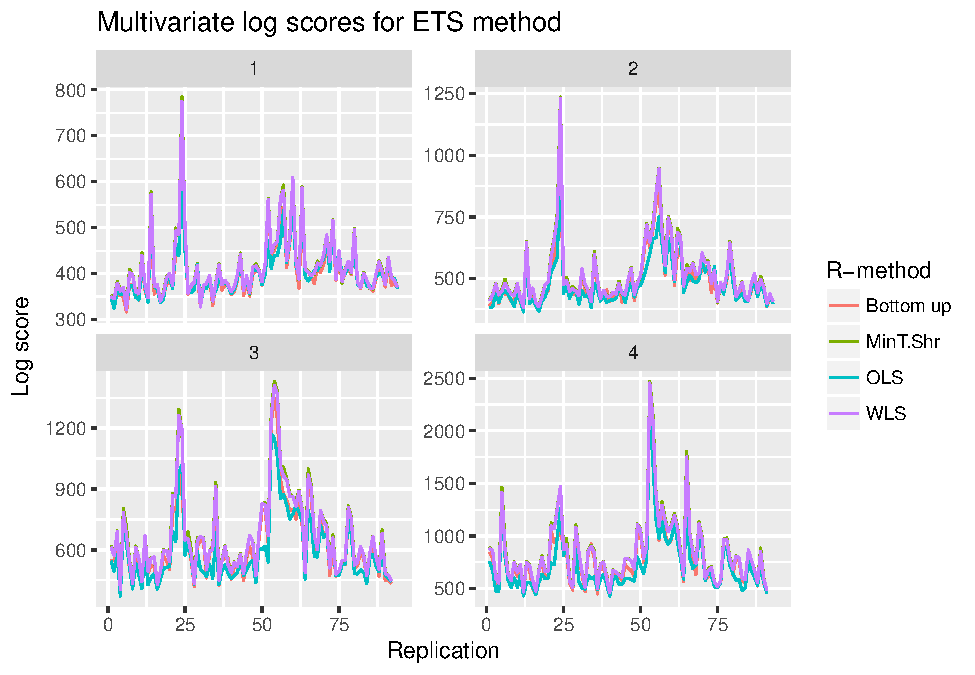
\includegraphics{Expenditure-approach-results_files/figure-latex/unnamed-chunk-14-1.pdf}

\begin{Shaded}
\begin{Highlighting}[]
\NormalTok{DF_MultiV }\OperatorTok\StringTok{ }\NormalTok{dplyr}\OperatorTok{::}\KeywordTok{select}\NormalTok{(}\OperatorTok{-}\StringTok{`}\DataTypeTok{Energy score}\StringTok{`}\NormalTok{, }\OperatorTok{-}\StringTok{`}\DataTypeTok{Variogram score}\StringTok{`}\NormalTok{) }\OperatorTok\StringTok{ }
\StringTok{  }\KeywordTok{filter}\NormalTok{(}\StringTok{`}\DataTypeTok{Log score}\StringTok{`} \OperatorTok{!=}\StringTok{ "NA"}\NormalTok{) }\OperatorTok\StringTok{ }
\StringTok{  }\KeywordTok{filter}\NormalTok{(}\StringTok{`}\DataTypeTok{F-method}\StringTok{`} \OperatorTok{==}\StringTok{ "ARIMA"}\NormalTok{) ->}\StringTok{ }\NormalTok{DF_Mult_LS_ARIMA}

\NormalTok{DF_Mult_LS_ARIMA }\OperatorTok\StringTok{ }\KeywordTok{ggplot}\NormalTok{(}\KeywordTok{aes}\NormalTok{(}\DataTypeTok{x =} \StringTok{`}\DataTypeTok{Replication}\StringTok{`}\NormalTok{, }\DataTypeTok{y =} \StringTok{`}\DataTypeTok{Log score}\StringTok{`}\NormalTok{, }\DataTypeTok{color =} \StringTok{`}\DataTypeTok{R-method}\StringTok{`}\NormalTok{)) }\OperatorTok{+}\StringTok{ }
\StringTok{  }\KeywordTok{geom_line}\NormalTok{() }\OperatorTok{+}\StringTok{ }\KeywordTok{facet_wrap}\NormalTok{(}\OperatorTok{~}\StringTok{`}\DataTypeTok{Forecast Horizon}\StringTok{`}\NormalTok{, }\DataTypeTok{scales =} \StringTok{"free_y"}\NormalTok{) }\OperatorTok{+}\StringTok{ }\KeywordTok{ggtitle}\NormalTok{(}\StringTok{"Multivariate log scores for ARIMA method"}\NormalTok{)}
\end{Highlighting}
\end{Shaded}

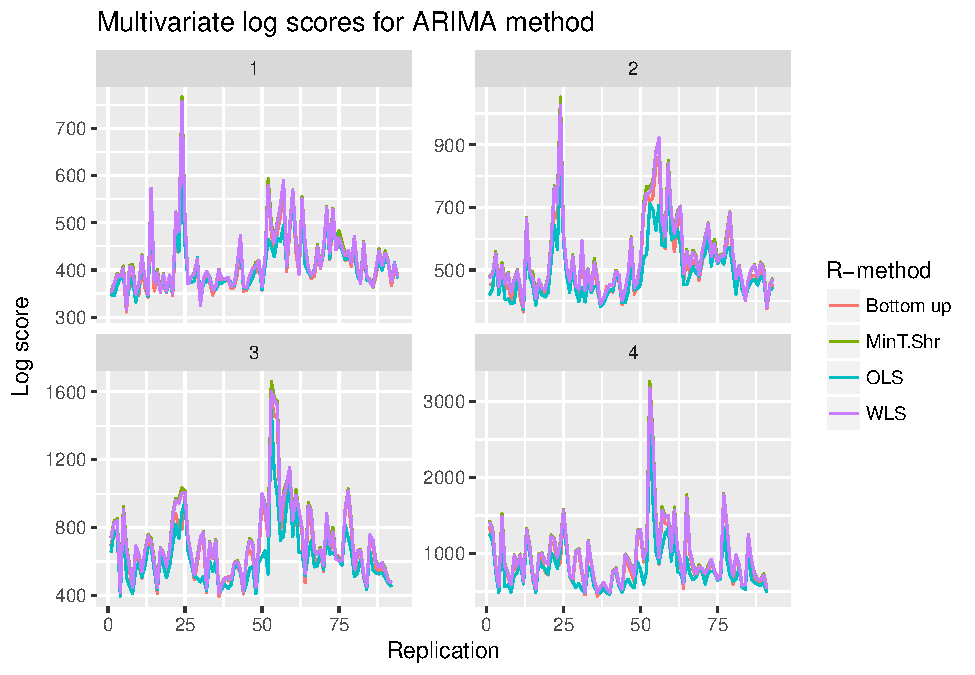
\includegraphics{Expenditure-approach-results_files/figure-latex/unnamed-chunk-14-2.pdf}

\subsection{Predictive ability of univariate forecast
distributions}\label{predictive-ability-of-univariate-forecast-distributions-1}

\subsubsection{Summary of GDP - The most aggregate
series}\label{summary-of-gdp---the-most-aggregate-series-2}

\begin{table}[H]
\centering
\begin{tabular}{l|r|r|r|r|r|r|r|r|r|r|r|r|r|r|r|r}
\hline
\multicolumn{1}{c|}{ } & \multicolumn{8}{|c|}{ETS} & \multicolumn{8}{|c}{ARIMA} \\
\cline{2-9} \cline{10-17}
\multicolumn{1}{c|}{ } & \multicolumn{4}{|c|}{CRPS} & \multicolumn{4}{|c|}{LS} & \multicolumn{4}{|c|}{CRPS} & \multicolumn{4}{|c}{LS} \\
\cline{2-5} \cline{6-9} \cline{10-13} \cline{14-17}
Method & 1 & 2 & 3 & 4 & 1 & 2 & 3 & 4 & 1 & 2 & 3 & 4 & 1 & 2 & 3 & 4\\
\hline
Benchmark & -130.00 & -58.82 & -12.94 & -4.28 & -5.53 & 11.24 & 29.09 & 36.32 & -133.49 & -49.65 & -20.19 & -8.14 & -4.15 & 15.78 & 31.60 & 37.55\\
\hline
Base & 0.00 & 0.00 & 0.00 & 0.00 & 0.00 & 0.00 & 0.00 & 0.00 & 0.00 & 0.00 & 0.00 & 0.00 & 0.00 & 0.00 & 0.00 & 0.00\\
\hline
OLS & 4.24 & 3.26 & 4.98 & 3.17 & -1.44 & -4.49 & -5.58 & -7.27 & 1.39 & 2.29 & 2.09 & 3.08 & -2.14 & -4.19 & -5.14 & -5.59\\
\hline
WLS & 5.87 & 3.75 & 7.82 & 2.85 & -2.85 & -7.56 & -7.39 & -9.31 & -0.22 & 1.83 & 1.00 & 2.05 & -3.73 & -5.77 & -5.50 & -5.18\\
\hline
MinT Shrink & 5.72 & 2.98 & 7.43 & 4.21 & -3.36 & -9.06 & -10.51 & -12.34 & -0.87 & -0.69 & -0.46 & 0.31 & -4.19 & -8.94 & -10.48 & -11.27\\
\hline
\end{tabular}
\end{table}

\subsubsection{Summary of all aggregate level
series}\label{summary-of-all-aggregate-level-series-2}

\begin{table}[H]
\centering
\begin{tabular}{l|r|r|r|r|r|r|r|r|r|r|r|r|r|r|r|r}
\hline
\multicolumn{1}{c|}{ } & \multicolumn{8}{|c|}{ETS} & \multicolumn{8}{|c}{ARIMA} \\
\cline{2-9} \cline{10-17}
\multicolumn{1}{c|}{ } & \multicolumn{4}{|c|}{CRPS} & \multicolumn{4}{|c|}{LS} & \multicolumn{4}{|c|}{CRPS} & \multicolumn{4}{|c}{LS} \\
\cline{2-5} \cline{6-9} \cline{10-13} \cline{14-17}
Method & 1 & 2 & 3 & 4 & 1 & 2 & 3 & 4 & 1 & 2 & 3 & 4 & 1 & 2 & 3 & 4\\
\hline
Benchmark & -70.80 & -55.79 & -22.73 & -5.75 & 11.95 & 1.74 & 12.44 & 22.13 & -66.95 & -55.09 & -23.68 & -9.08 & 11.26 & 1.09 & 11.34 & 19.55\\
\hline
Base & 0.00 & 0.00 & 0.00 & 0.00 & 0.00 & 0.00 & 0.00 & 0.00 & 0.00 & 0.00 & 0.00 & 0.00 & 0.00 & 0.00 & 0.00 & 0.00\\
\hline
OLS & 2.25 & 1.65 & 1.12 & 0.74 & -1.35 & -3.26 & -4.78 & -4.81 & 2.07 & 0.52 & 0.47 & 0.11 & -0.68 & -3.28 & -4.07 & -4.36\\
\hline
WLS & 4.13 & 3.80 & 2.27 & 0.97 & -11.85 & -8.79 & -13.68 & -17.23 & 0.89 & -0.62 & 0.29 & -0.41 & -12.82 & -8.85 & -12.79 & -16.23\\
\hline
MinT Shrink & 4.78 & 4.90 & 2.65 & 1.15 & -12.91 & -9.45 & -15.31 & -19.68 & 1.54 & -0.96 & 0.19 & -0.98 & -14.56 & -10.49 & -15.12 & -19.28\\
\hline
\end{tabular}
\end{table}

\subsubsection{Summary of all disaggregate
series}\label{summary-of-all-disaggregate-series-2}

\begin{table}[H]
\centering
\begin{tabular}{l|r|r|r|r|r|r|r|r|r|r|r|r|r|r|r|r}
\hline
\multicolumn{1}{c|}{ } & \multicolumn{8}{|c|}{ETS} & \multicolumn{8}{|c}{ARIMA} \\
\cline{2-9} \cline{10-17}
\multicolumn{1}{c|}{ } & \multicolumn{4}{|c|}{CRPS} & \multicolumn{4}{|c|}{LS} & \multicolumn{4}{|c|}{CRPS} & \multicolumn{4}{|c}{LS} \\
\cline{2-5} \cline{6-9} \cline{10-13} \cline{14-17}
Method & 1 & 2 & 3 & 4 & 1 & 2 & 3 & 4 & 1 & 2 & 3 & 4 & 1 & 2 & 3 & 4\\
\hline
Benchmark & -21.37 & -6.39 & -22.58 & -19.45 & 21.03 & 36.61 & 17.12 & 12.00 & -18.89 & -3.17 & -18.96 & -16.45 & 27.52 & 45.46 & 18.07 & 14.67\\
\hline
Base & 0.00 & 0.00 & 0.00 & 0.00 & 0.00 & 0.00 & 0.00 & 0.00 & 0.00 & 0.00 & 0.00 & 0.00 & 0.00 & 0.00 & 0.00 & 0.00\\
\hline
OLS & -4.64 & -6.43 & -6.11 & -7.67 & 12.98 & 21.02 & 3.57 & 6.95 & -3.16 & -3.09 & -4.04 & -4.66 & 21.14 & 33.84 & 4.57 & 10.33\\
\hline
WLS & -0.06 & -1.30 & -1.58 & -3.08 & -3.02 & -3.76 & -2.94 & -2.91 & 0.44 & 0.13 & -0.36 & -0.65 & -2.22 & -2.34 & -2.39 & -2.07\\
\hline
MinT Shrink & 0.64 & -1.56 & -2.05 & -3.54 & -4.12 & -5.36 & -4.20 & -3.92 & 0.54 & 0.19 & -0.79 & -1.52 & -3.60 & -4.06 & -3.84 & -3.37\\
\hline
\end{tabular}
\end{table}

\subsubsection{Summary of all series in the
hierarchy}\label{summary-of-all-series-in-the-hierarchy-2}

\begin{table}[H]
\centering
\begin{tabular}{l|r|r|r|r|r|r|r|r|r|r|r|r|r|r|r|r}
\hline
\multicolumn{1}{c|}{ } & \multicolumn{8}{|c|}{ETS} & \multicolumn{8}{|c}{ARIMA} \\
\cline{2-9} \cline{10-17}
\multicolumn{1}{c|}{ } & \multicolumn{4}{|c|}{CRPS} & \multicolumn{4}{|c|}{LS} & \multicolumn{4}{|c|}{CRPS} & \multicolumn{4}{|c}{LS} \\
\cline{2-5} \cline{6-9} \cline{10-13} \cline{14-17}
Method & 1 & 2 & 3 & 4 & 1 & 2 & 3 & 4 & 1 & 2 & 3 & 4 & 1 & 2 & 3 & 4\\
\hline
Benchmark & -50.77 & -35.31 & -22.68 & -9.74 & 17.94 & 27.04 & 15.46 & 16.15 & -47.50 & -33.24 & -22.13 & -11.32 & 22.25 & 34.67 & 15.72 & 16.57\\
\hline
Base & 0.00 & 0.00 & 0.00 & 0.00 & 0.00 & 0.00 & 0.00 & 0.00 & 0.00 & 0.00 & 0.00 & 0.00 & 0.00 & 0.00 & 0.00 & 0.00\\
\hline
OLS & -0.54 & -1.70 & -1.20 & -1.71 & 8.03 & 14.31 & 0.51 & 2.22 & -0.05 & -1.00 & -1.01 & -1.33 & 13.99 & 24.84 & 1.52 & 4.62\\
\hline
WLS & 2.43 & 1.69 & 1.03 & -0.21 & -6.14 & -5.18 & -6.82 & -8.58 & 0.71 & -0.30 & 0.08 & -0.48 & -5.63 & -3.93 & -6.09 & -7.63\\
\hline
MinT Shrink & 3.10 & 2.22 & 1.14 & -0.22 & -7.14 & -6.50 & -8.24 & -10.19 & 1.14 & -0.48 & -0.13 & -1.14 & -7.14 & -5.58 & -7.81 & -9.54\\
\hline
\end{tabular}
\end{table}

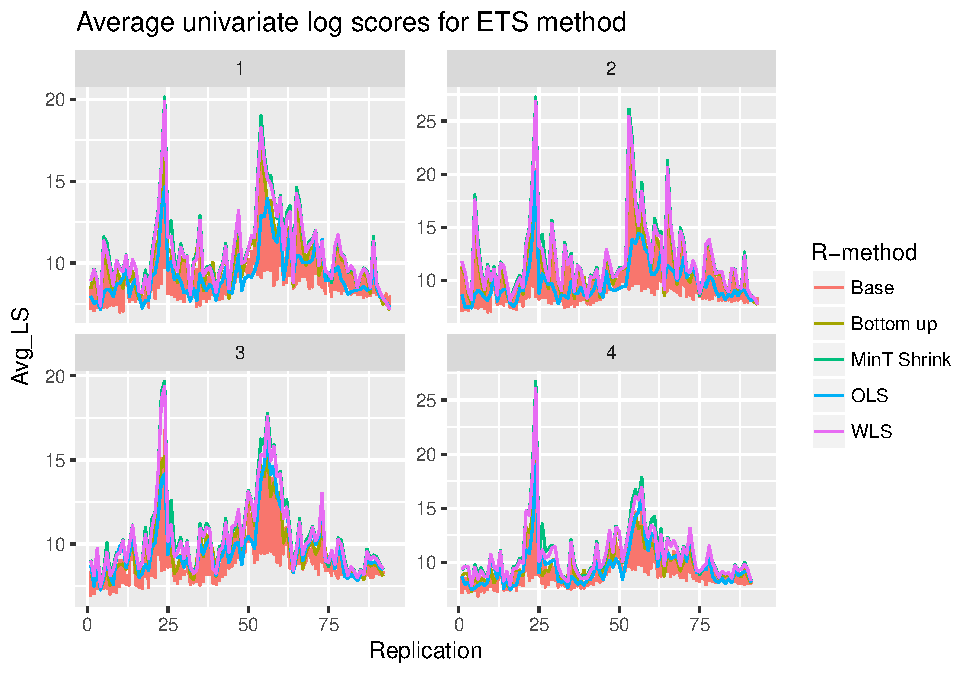
\includegraphics{Expenditure-approach-results_files/figure-latex/unnamed-chunk-18-1.pdf}
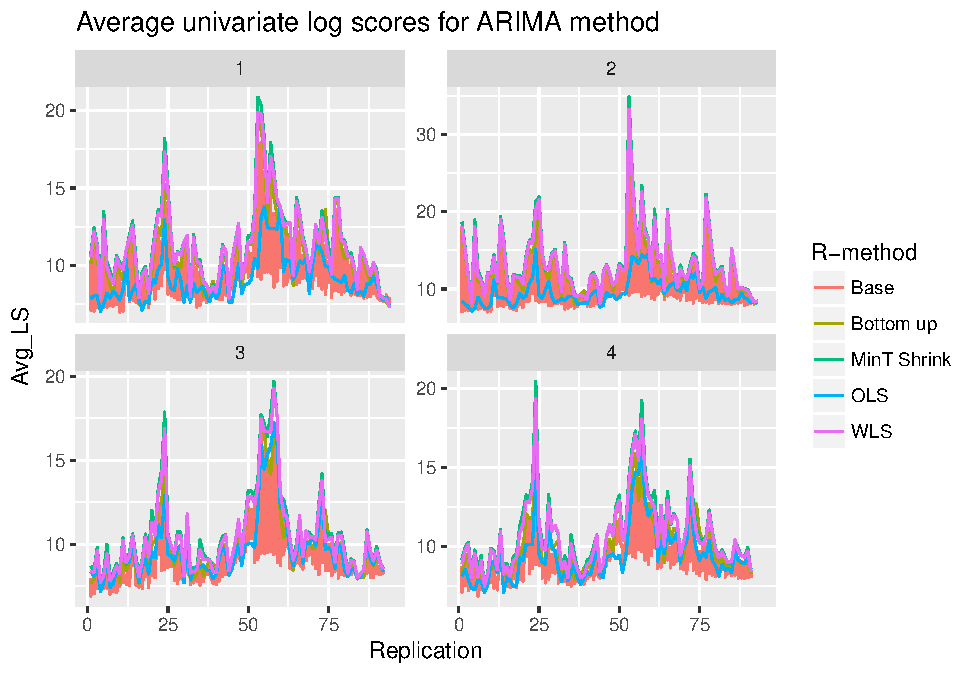
\includegraphics{Expenditure-approach-results_files/figure-latex/unnamed-chunk-18-2.pdf}


\end{document}
